\documentclass{scrartcl}
\usepackage[utf8]{inputenc}
\usepackage{graphicx}
\usepackage{adjustbox}
\usepackage{amsmath}
\usepackage{float}
\usepackage{siunitx}
\sisetup{
  per-mode=symbol,
  separate-uncertainty
}
\usepackage{hyperref}
\hypersetup{
    colorlinks=true,
    linkcolor=blue,
    filecolor=magenta,      
    urlcolor=cyan,    
    }
\usepackage{authblk}

\usepackage{minted}

\title{CGL-sheet07}

\author[1]{Robin Kühnberger}
\author[2]{Felix Naraschewski}

\affil[1]{University Stuttgart}
\affil[2]{University Stuttgart}

\date{\today}

\begin{document}
\maketitle
\tableofcontents

\section{Aufgabe 1}

\begin{figure}[H]
	\centering
	\adjincludegraphics[max width=1\textwidth]{Pasted image 20251202223119.png}
	\caption{Artikel mit Metadaten}
	\label{img:01}
\end{figure}

\begin{figure}[H]
	\centering
	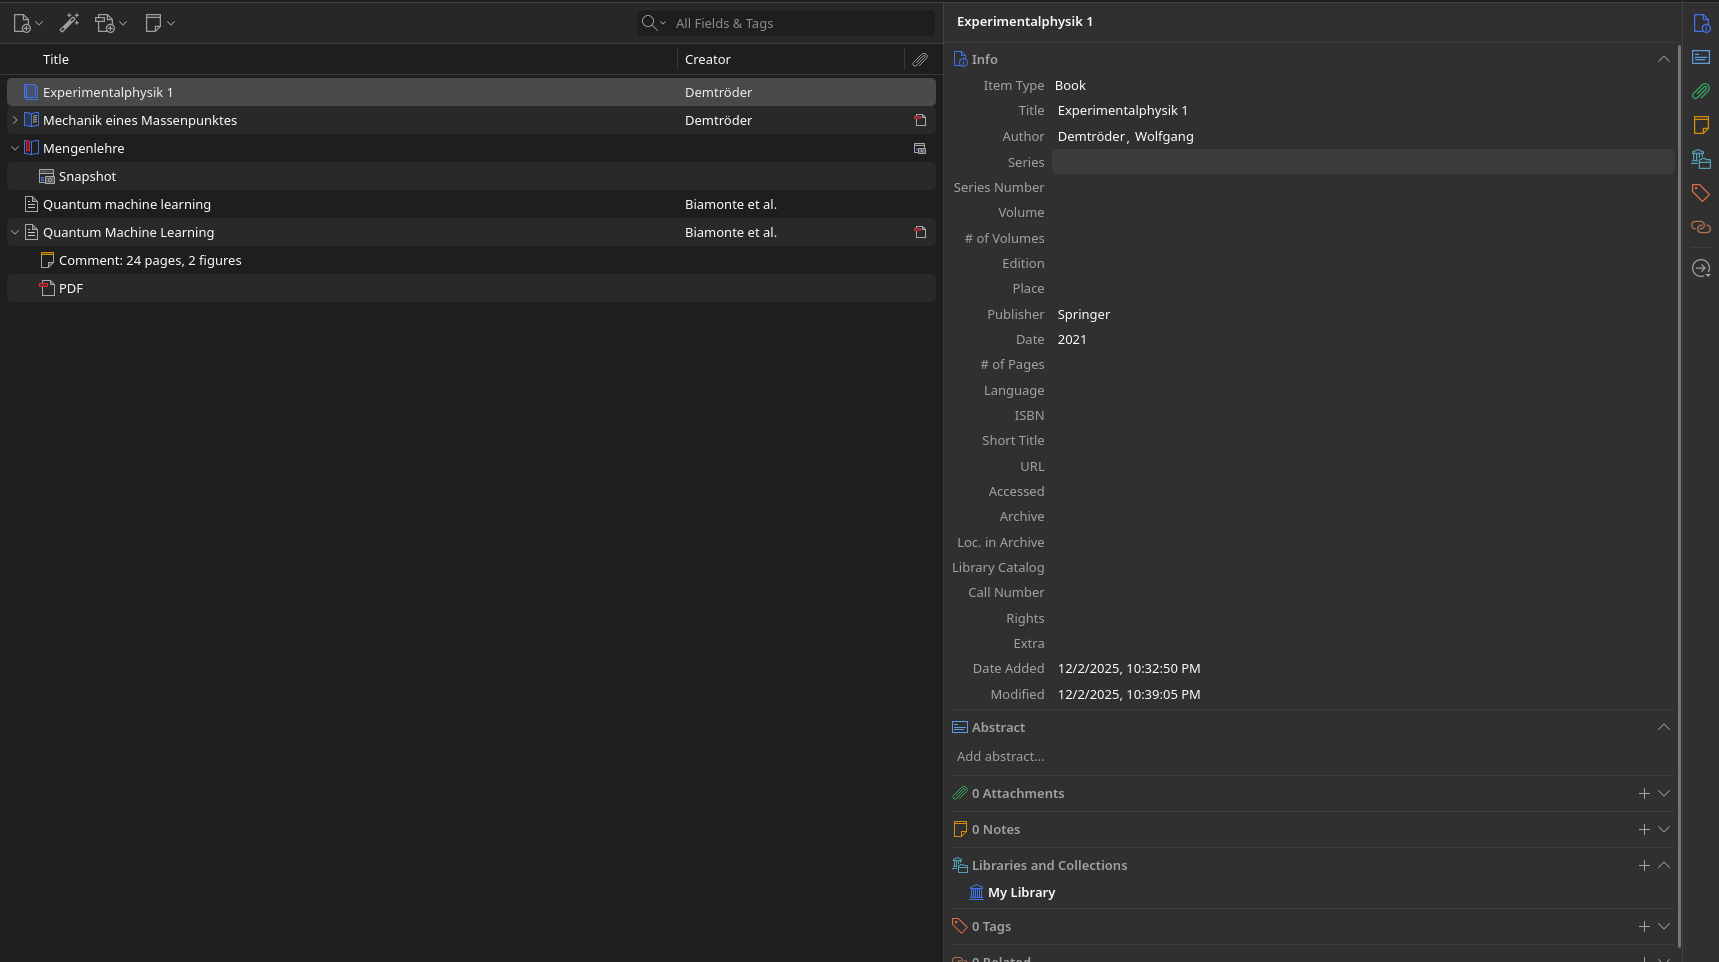
\includegraphics[width=1\textwidth]{Pasted image 20251202224038.png}
	\caption{Experimentalphysik 1 Buch}
	\label{img:02}
\end{figure}

\subsection{Bib referenzen}
\cite{biamonte_quantum_2017}
\cite{demtroder_experimentalphysik_2021}

\section{List Comprehension}

\inputminted[breaklines]{python3}{Python/list_comprehension.py}

\begin{figure}[H]
	\centering
	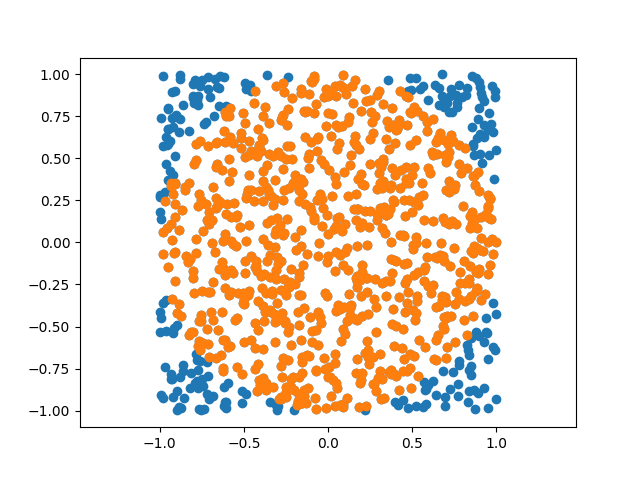
\includegraphics[width=1\textwidth]{Python/pi_montecarlo_plot.png}
	\caption{Scatter Plot}
	\label{img:03}
\end{figure}

\begin{equation}
	\begin{aligned}
		\text{Verhätnis}=\frac{N_{\text{filtered}}}{N} \approx & \frac{A_{\text{Kreis}}}{A_{\text{Quadrat}}} \\
		\frac{(1)^{2}\cdot \pi}{2^{2}}=                        & \frac{\pi}{4}
		\label{eq:gleichung0}
	\end{aligned}
\end{equation}



\section{Dateien lesen und Daten plotten}

\inputminted[breaklines]{python3}{Python/read_data.py}

\begin{figure}[H]
	\centering
	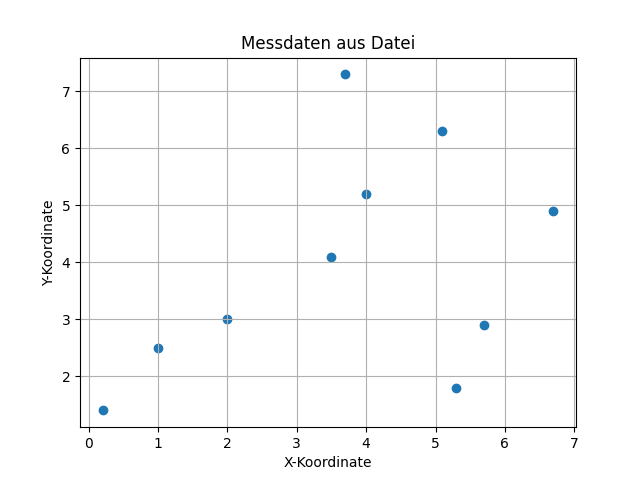
\includegraphics[width=1\textwidth]{Python/messdaten_plot.png}
	\caption{Scatter Plot}
	\label{img:04}
\end{figure}

\section*{Quellen}
\bibliographystyle{plain}
\bibliography{bibliography.bib}

\listoffigures
%\listoftables

\end{document}